\subsection{Discuss the symmetry properties of the He wave functions and show which solutions are possible due to the Pauli principle.}


\paragraph{Generelt omkring helium grundtilstanden -- Good to know:} Helium består af to elektroner, som er i banebevægelse omkring den positive kerne. Schrödingerligningen for de to elektroner i et Coulombpotential fra ladningen $Ze$ fra kernen vil være
\begin{align}
    \left(H_{kin,1} + H_{kin,2} + H_{pot}\right)\psi &= \left\{\frac{-\hbar^2}{2m}\nabla_1^2 + \frac{-\hbar^2}{2m}\nabla_2^2 + \frac{e^2}{4\pi\epsilon_0} \left(-\frac{Z}{r_1} - \frac{Z}{r_2} + \frac{1}{r_{12}}\right)\right\} = E\psi \: ,
\end{align}
hvor $r_{12} = |\Vec{r}_1 - \Vec{r}_2|$ er afstanden mellem de to elektroner, hvorfor deres frastødning er proportionel til $1/r_{12}$. I øjeblikket bliver denne frastødning negligeret, hvorved Schrödingerligningen kan skrives som
\begin{align}
    \left(H_1 + H_2\right)\psi &= E^{(0)}\psi \: ,
\end{align}
hvor
\begin{align}
    H_i &\equiv \frac{-\hbar^2}{2m}\nabla_i^2 - \frac{Ze^2}{4\pi\epsilon_0 r_i} \: , \quad \forall i = 1,\,2 \: .
\end{align}
Skrives bølgefunktionen nu som et produkt af bølgefunktionen for hver af elektronerne, $\psi = \psi(1)\psi(2)$, fås
\begin{align}
    H_i\psi(i) &= E_i\psi(i) \: , \quad \forall i = 1,\,2 \: .
\end{align}
Løsningerne til disse enkeltelektronligninger er hydrogenbølgefunktioner med energier givet ved Rydbergformlen. Den totale energi heraf bliver $E^{(0)} = E_1 + E_2 = \SI{-109}{\eV}$.\\

Tilføjes energien fra frastødningen som en perturbation fås energien $E(1s^2) =  \SI{-109}{\eV} + \SI{34}{\eV} = \SI{-75}{\eV}$, hvor energien fra frastødningen er $E^{(1)} = \SI{34}{\eV}$. Det kræver altså $\SI{-75}{\eV}$ at fjerne begge elektroner fra helium og efterlade $\text{He}^{++}$ -- dette kaldes den \emph{anden ioniseringsenergi}. For at gå fra $\text{He}^{+}$ til $\text{He}^{++}$ kræver det $\SI{54.4}{\eV}$. Estimeret må \emph{første ioniseringsenergi} derved være $IE(\text{He}) \simeq \SI{75}{\eV} - \SI{54}{\eV} = \SI{21}{\eV}$. Men energien af frastødningen er ikke lille i sammenlignet med bindingsenergien, hvorfor perturbationen har en signifikant betydning for bølgefunktionerne. Benytter man i stedet variationsmetoden\footnote{This is a stadndard quantum mechanical technique whose mathematical details are given in quantum texts. The essential principle of this technique is to find an expression for the energy in terms of a parameter -- an effective atomic number in the case of helium -- and then minimize the enrgy with respect to this parameter, i.e. study the variation in the energy as a function of the chosen parameter.}, kan man komme meget tæt på de reelle energier ($\sim\SI{2}{\percent}$ forskel til de eksperimentelle resultater). Her gør man brug af et gæt på den totale bølgefunktion af helium, som værende to $1s$-hydrogenbølgefunktioner ganget sammen, og vi lader kernes ladning være en kontinuert parameter, som vi så kan minimere, idet forventningsværdien af Hamiltonoperatoren af denne bølgefunktion, altid vil være større end eller lig med grundtilstandsenergien (alt efter hvor godt et gæt, som vi får). Ved at minimere forventningsværdien af Hamiltonoperatoren får vi en effektiv kerneladning mindre end $2e$, som er heliums kerneladning, hvorfor vi ser dette som værende en skærmning (eng. shielding) af kernen.\\



\paragraph{Exciterede tilstande - Actually answer to question:} Vi betragter to elektroner i hhv. tilstanden 1s (altså $n=1$ og $l=0$) og en vilkårlig tilstand $n,\,l$. Med en stadig negligeret interaktion mellem de to elektroner ser vi stadig bølgefunktionen som værende et produkt af bølgefunktionen for hver af elektronerne, $\psi = \psi(1)\psi(2)$, hvorfor
\begin{align}
    \psi_\text{sp}(1,2) &= \psi_{1s}(1)\psi_{nl}(2) \: , \quad \text{og} \\
    \psi_\text{sp}(2,1) &= \psi_{1s}(2)\psi_{nl}(1) \: ,
\end{align}
da vi har tale om identiske partikler. Disse er enrgimæssigt udartede (eng. energetically degenerate), men i stdet for at gå i gang med udartet perturbationsteori kan man tænkte smart og undgå perturbationsteori ved at gøre brug af de rigtige argumenter.

Idet at vi har tale om identiske partikler må det gøre sig gældende, at
\begin{align}
    \abs{\psi_\text{sp}(1,2)}^2 &= \abs{\psi_\text{sp}(2,1)}^2 \: ,
\end{align}
og benytter vi \emph{permutationsoperatoren} (eng. exchange operator) $P$, hvorom det gælder, at
\begin{align}
    P^2 \psi(1,2) &= \psi(1,2) \: , \quad \text{og} \label{eq:Q11_ExchangeOperatorDefinitions1} \\
    P \psi(1,2) &= \psi(2,1) \: ,\label{eq:Q11_ExchangeOperatorDefinitions2}
\end{align}
og som har egenvektorfunktionerne
\begin{align}
    P^2 \psi &= p^2 \psi \: , \quad \text{og} \label{eq:Q11_ExchangeOperatorEingenValueFunctions1} \\
    P \psi &= p \psi \: , \label{eq:Q11_ExchangeOperatorEingenValueFunctions2}
\end{align}
da får vi, at
\begin{align}
    \abs{\psi_\text{sp}(1,2)}^2 &= \abs{\psi_\text{sp}(2,1)}^2
    = \abs{P\psi_\text{sp}(1,2)}^2
    = \abs{p\psi_\text{sp}(1,2)}^2
    = \abs{p}^2 \abs{\psi_\text{sp}(1,2)}^2 \nonumber\\
    \Rightarrow \abs{p}^2 &= 1 \: .
\end{align}
Dette betyder, at brugen af permutationsoperatoren ikke kan ændre amplituden af bølgefunktionen, som den benyttes på, hvorfor den må ændre fasen i stedet, hvilken er givet ved
\begin{align} \label{eq:Q11_FaseskiftP}
    p &= \exp{i\phi} \: ,
\end{align}
hvor $\phi$ er vinklen for faseskiftet.

Sammenligner vi nu \cref{eq:Q11_ExchangeOperatorDefinitions1} med \cref{eq:Q11_ExchangeOperatorEingenValueFunctions1} kan det ses, at
\begin{align}
    \psi(1,2) &= P^2 \psi(1,2) = p^2 \psi(1,2) \nonumber\\
    \Rightarrow p^2 = 1 \: .
\end{align}
Benytter vi nu dette med \cref{eq:Q11_FaseskiftP}, så fås
\begin{align}
    1 &= p^2 = \left(\exp{i\phi}\right)^2 = \exp{2i\phi} \nonumber\\
    \Rightarrow \phi &= k\pi \: , \quad \forall k \in \mathbb{N}_0 \: .
\end{align}
Dette indsættes nu i \cref{eq:Q11_FaseskiftP}, hvorved vi kan finde $p$
\begin{align}
    p &= \exp{i\phi} =
        \begin{cases}
            \exp(i \cdot 0) = \exp(0) = 1 \\
            \exp(i\pi) = \cos(\pi) + i\sin(\pi) = \cos(\pi) = -1
        \end{cases} \: ,
\end{align}
altså $p = \pm 1$.

Ved at benytte, at $p = \pm 1$, så kan det ses, at
\begin{align} \label{eq:Q11_SymmetrikravTilBoelgefunktionerne}
    \psi(1,2) &= P\psi(2,1) = p\psi(2,1) = \pm \psi(2,1) \: .
\end{align}
Vi kan altså have bølgefunktioner, som er symmetriske ($+$) eller antisymmetriske ($-$) under ombytning. For at opfylde symmetrikravene i \cref{eq:Q11_SymmetrikravTilBoelgefunktionerne} dannes to bølgefunktioner for de to elektroner
\begin{align}
    \psi^S(1,2) &= \frac{1}{\sqrt{2}} \left\{\psi_{1s}(1)\psi_{nl}(2) + \psi_{1s}(2)\psi_{nl}(1)\right\} \: , \text{og} \\
    \psi^S(1,2) &= \frac{1}{\sqrt{2}} \left\{\psi_{1s}(1)\psi_{nl}(2) - \psi_{1s}(2)\psi_{nl}(1)\right\} \: ,
\end{align}
hvor $S$ og $A$ angiver om der er tale om den hhv. symmetriske eller antisymmetriske bølgefunktion.\\

Ovenfor har vi behandlet de rummelige bølgefunktioner, men vi ved, at elektronen har et spin, som også skal medtages i den totale bølgefunktion, $\Psi = \psi(\Vec{r}) \otimes \chi(\Vec{s})$, for at denne beskriver systemet. De mulige spinbølgefunktioner for to spin-$1/2$ partikler er
\begin{align}
    \ket{\uparrow\uparrow} \: , \quad \ket{\uparrow\downarrow} \: , \quad \ket{\downarrow\uparrow} \: , \quad \text{og} \quad \ket{\downarrow\downarrow} \: .
\end{align}
Disse skal være egenfunktioner for $\Vec{s}^2$, hvilket kun gør sig gældende for $\ket{\uparrow\uparrow}$ og $\ket{\downarrow\downarrow}$, hvorfor de to andre ''redefineres'', således at vi får de følgende symmetriske og antisymmetriske spinbølgefunktioner
\begin{align}
    \chi^S &= \ket{\uparrow\uparrow} \: , \qquad \qquad \qquad \quad \text{hvor} \quad m_s = 1 \: , \\
    \chi^S &= \ket{\downarrow\downarrow} \: , \qquad \qquad \qquad \quad \text{hvor} \quad m_s = -1 \: , \\
    \chi^S &= \frac{1}{\sqrt{2}} \Big(\ket{\uparrow\downarrow} + \ket{\downarrow\uparrow}\Big) \: , \,\quad \text{hvor} \quad m_s = 0 \: , \\
    \chi^A &= \frac{1}{\sqrt{2}} \Big(\ket{\uparrow\downarrow} - \ket{\downarrow\uparrow}\Big) \: , \,\quad \text{hvor} \quad m_s = 0 \: .
\end{align}
Triplettilstanden (de symmetriske spinbølgefunktioner) har altså $s = 1$, mens singlettilstanden (den antisymmetriske spinbølgefunktion) har $s = 0$.


\paragraph{Mulige bølgefunktioner respekterende Paulis udelukkelsesprincip:} Paulis udelukkelseprincip siger i sin korthed, at den totale bølgefunktion for et system med mere end én identisk fermion altid skal være antisymmetrisk under ombytning af disse fermioner. Det vil sige, at de mulige totalbølgefunktioner vil være
\begin{align}
    \Psi &= \psi^S \otimes \chi^A \: , \quad \text{og} \\
    \Psi &= \psi^A \otimes \chi^S \: ,
\end{align}
hvor den første bølgefunktion vil give en singlettilstand, da $S = 0$, hvormed multipliciten\footnote{Se termsymbol i disposition 14.} er $2S + 1 = 1$, og den anden mulighed giver en triplettilstand, da $S = 1$, hvormed multipliciteten er $2S + 1 = 3$.

Kigger vi på grundtilstanden i helium er der kun én mulig bølgefunktion
\begin{align}
    \Psi &= \psi^S \otimes \chi^A = \frac{1}{2} \Big\{\psi_{1s}(1)\psi_{nl}(2) + \psi_{1s}(2)\psi_{nl}(1)\Big\}\Big(\ket{\uparrow\downarrow} - \ket{\downarrow\uparrow}\Big) \: ,
\end{align}
idet at en antisymmetrisk bølgefunktion ville give $0$, da $\psi_{1s}(1)\psi_{1s}(2) =\psi_{1s}(2)\psi_{1s}(1)$.

Kigger vi nu i stedet på helium med én exciteret elektron, således at $n_1 = 2$, mens $n_2 = 1$ og $l_2 = 0$, så vil de følgende tilstande være mulige
\begin{align}
    2^1S_0 &\quad \left(l_1 = 0,\: m_{l_1} = 0, \: m_{s_1} = -\frac{1}{2}, \: J = 0\right) \: , \\
    2^1P_1 &\quad \left(l_1 = 1,\: m_{l_1} = 0,\pm1, \: m_{s_1} = -\frac{1}{2}, \: J = 1\right) \: , \\
    2^3S_1 &\quad \left(l_1 = 0,\: m_{l_1} = 0, \: m_{s_1} = \frac{1}{2}, \: J = 1\right) \: , \\
    2^3P_0 &\quad \left(l_1 = 1,\: m_{l_1} = -1, \: m_{s_1} = \frac{1}{2}, \: J = 0\right) \: , \\
    2^3P_1 &\quad \left(l_1 = 1,\: m_{l_1} = 0, \: m_{s_1} = \frac{1}{2}, \: J = 1\right) \: , \\
    2^3P_2 &\quad \left(l_1 = 1,\: m_{l_1} = 1, \: m_{s_1} = \frac{1}{2}, \: J = 2\right) \: ,
\end{align}
hvilke kan ses af \cref{fig:Q11_SingletOgTripletTilstandeIHelium}.

\begin{figure}[!h]
    \centering
    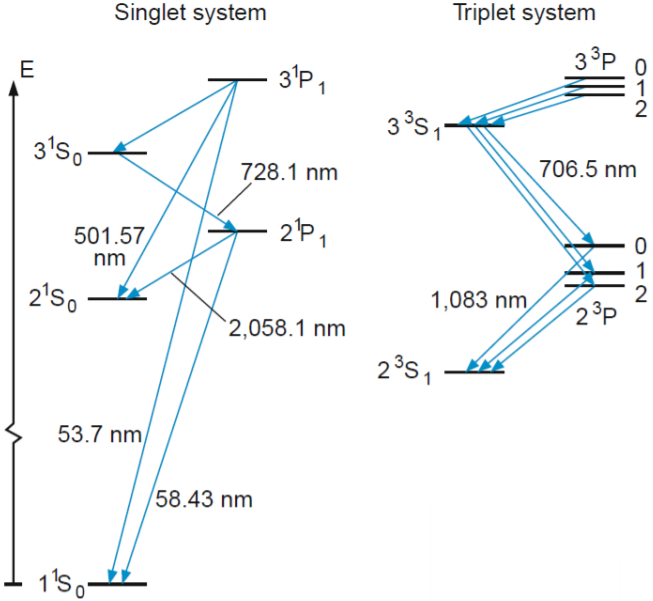
\includegraphics[width=0.7\textwidth]{Q11/images/SingletOgtripletTilstandeIHelium.PNG}
    \caption{De tilladte overgange mellem niveauer i helium styres af udvagsreglerne $\Delta S = 0$, som undgår overgange mellem singlet- og tripletsystemet, og $\Delta L = \pm 1$. Siden at der ikke er overgange mellem singlet- og tripletsystemet er det smart at tegne disse hver for sig, og det blev tidligere troet, at disse var to forskellige typer af helium, som blev kaldt hhv. ortohelium og parahelium.}
    \label{fig:Q11_SingletOgTripletTilstandeIHelium}
\end{figure}

På \cref{fig:Q11_SingletOgTripletTilstandeIHelium} kan der bemærkes lidt forskelligt:
\begin{itemize}
    \item Der findes ikke et $(1s)(1s)$ grundtilstand i triplettilstnden, da dette ville give $\psi^S = 0$.
    \item For $L = 0$ (S-obitaltilstande) forekommer der ikke nogen energiopsplitning til ''triplettilstande''.
    \item For $L \ne 0$ kommer opsplitningerne af finstrukturen, som opsplitter mht. $J$.
    \item Der findes ingen overgange mellem singlet- og tripletsystemerne, da udvalgsreglen omkring $\Delta S = 0$ forbyder at gå mellem $S = 0$ og $S = 1$ tilstandene.
    \begin{itemize}
        \item Tidligere blev det troet, at de to systemer var to forskellige typer af helium (da disse to systemer aldrig skiftede mellem hinanden), hvor singletsystemet blev kaldt \emph{ortohelium}, og tripletsystemet blev kaldt \emph{parahelium}.
    \end{itemize}
\end{itemize}